\chapter{The C Programming Language}

\epigraph{If you want to teach systems, don't drum up the programmers, sort the issues, and make PRs. Instead, teach them to yearn for the vast and endless C.}{Antoine de Saint-Exup\'{e}ry (With edits)}

Note: This chapter is long and goes into a lot of detail. Feel free to gloss over parts with which you have experience in.

C is the de-facto programming language to do serious system serious programming.
Why?
Most kernels have their API accessible through C.
The Linux kernel \cite{Love} and the XNU kernel \cite{xnukernel} of which MacOS is based on are written in C and have C API - Application Programming Interface.
The Windows Kernel uses C++, but doing system programming on that is much harder on windows that UNIX for novice system programmers.
C doesn't have abstractions like classes and Resource Acquisition Is Initialization (RAII) to clean up memory.
C also gives you much more of an opportunity to shoot yourself in the foot, but it lets you do things at a much more fine-grained level.

\section{History of C}

C was developed by \gls{Dennis Ritchie} and \gls{Ken Thompson} at \gls{Bell Labs} back in 1973 \cite{Ritchie:1993:DCL:155360.155580}.
Back then, we had gems of programming languages like \gls{Fortran}, \gls{ALGOL}, and \gls{LISP}.
The goal of C was two fold.
Firstly, it was made to target the most popular computers at the time, such as the \gls{PDP-7}.
Secondly, it tried to remove some of the lower level constructs (managing \gls{registers}, and programming assembly for \gls{jumps}), and create a language that had the power to express programs procedurally (as opposed to mathematically like LISP) with readable code.
All this while still having the ability to interface with the operating system.
It sounded like a tough feat.
At first, it was only used internally at Bell Labs along with the UNIX operating system.

The first "real" standardization was with \gls{Brian Kernighan} and Dennis Ritchie's book \cite{kernighan1988c}.
It is still widely regarded today as the only \gls{portable} set of C instructions.
The K\&R book is known as the de-facto standard for learning C.
There were different standards of C from \gls{ANSI} to \gls{ISO}, though ISO largely won out as a language specification.
We will be mainly focusing on is the \gls{POSIX} C library which extends ISO.
Now to get the elephant out of the room, the \gls{Linux kernel} is not entirely POSIX compliant.
Mostly, this is so because the Linux developers didn't want to pay the fee for compliance.
It is also because they did not want to be fully compliant with a multitude of different standards because that meant increased development costs to maintain compliance.

We will aim to use C99, as it is the standard that most computers recognize, but sometimes use some of the newer C11 features.
We will also talk about some off-hand features like \keyword{getline} because they are so widely used with the \gls{GNU C library}.
We'll begin by providing a fairly comprehensive overview of the language with language facilities.
Feel free to gloss over if you have already worked with a C based language.


\subsection{Features}

\begin{itemize}
	\item Speed. There is very little separating you and the system.
	\item Simplicity.
    C and its standard library comprise a simple set of portable functions.
	\item Manual Memory Management.
    C gives you the ability you manage your memory.
    However, this can bite you if you have memory errors.
  \item Ubiquity.
    Through foreign function interfaces (FFI) and language bindings of various types, most other languages can call C functions, and vice versa.
    The standard library is also everywhere.
    C has stood the test of time as a popular language, and it doesn't look like it is going anywhere.
\end{itemize}



\section{Crash course introduction to C}

The canonical way to start learning C is by starting with the \gls{hello world} program.
The original example that Kernighan and Ritchie proposed way back when hasn't changed.

\begin{lstlisting}[language=C]
#include <stdio.h>
int main(void) {
  printf("Hello World\n");
  return 0;
}
\end{lstlisting}

\begin{enumerate}
	\item The \keyword{\#include} directive takes the file \keyword{stdio.h} (which stands for \textbf{st}an\textbf{d}ard \textbf{i}nput and \textbf{o}utput) located somewhere in your operating system, copies the text, and substitutes it where the \keyword{\#include} was.
	\item The \keyword{int main(void)} is a function declaration.
    The first word \keyword{int} tells the compiler the return type of the function.
    The part before the parenthesis (\keyword{main}) is the function name.
    In C, no two functions can have the same name in a single compiled program, although shared libraries may be able.
    Then, the parameter list comes after.
    When we provide the parameter list for regular functions \keyword{(void)} that means that the compiler should produce an error if the function is called with a non-zero number of arguments.
    For regular functions having a declaration like \keyword{void func()} means that the function can be called like \keyword{func(1, 2, 3)}, because there is no delimiter.
    \keyword{main} is a special function.
    There are many ways of declaring \keyword{main} but the standard ones are \keyword{int main(void)}, \keyword{int main()}, and \keyword{int main(int argc, char *argv[])}.
	\item \keyword{printf("Hello World\n");} is what a function call.
    \keyword{printf} is defined as a part of \keyword{stdio.h}.
    The function has been compiled and lives somewhere else on our machine - the location of the C standard library.
    Just remember to include the header and call the function with the appropriate parameters (a string literal \keyword{"Hello World\n"}).
    If the newline isn't included, the buffer will not be flushed (i.e. the write will not complete immediately).
	\item \keyword{return 0}.
    \keyword{main} has to return an integer.
    By convention, \keyword{return 0} means success and anything else means failure.
    Here are some exit codes / statuses with special meaning: \url{http://tldp.org/LDP/abs/html/exitcodes.html}.
    In general, assume 0 means success.
\end{enumerate}

\begin{lstlisting}[language=bash]
$ gcc main.c -o main
$ ./main
Hello World
$
\end{lstlisting}

\begin{enumerate}
\item \keyword{gcc} is short for the \gls{GNU Compiler Collection} which has a host of compilers ready for use.
  The compiler infers from the extension that you are trying to compile a .c file.
\item \keyword{./main} tells your shell to execute the program in the current directory called main.
  The program then prints out "hello world".
\end{enumerate}

If systems programming was as easy as writing hello world though, our jobs would be much easier.

\subsection{Preprocessor}

What is the \gls{preprocessor}?
Preprocessing is a copy and paste operation that the compiler performs \textbf{before} actually compiling the program.
The following is an example of substitution

\begin{lstlisting}[language=C]
// Before preprocessing
#define MAX_LENGTH 10
char buffer[MAX_LENGTH]

// After preprocessing
char buffer[10]
\end{lstlisting}

There are side effects to the preprocessor though.
One problem is that the preprocessor needs to be able to \gls{tokenize} properly, meaning trying to redefine the internals of the C language with a preprocessor may be impossible.
Another problem is that they can't be \gls{nested} infinitely - there is a bounded depth where they need to stop.
Macros are also just simple text substitutions, without semantics.
For example, look at what can happen if a macro tries to perform an inline modification.

\begin{lstlisting}[language=C]
#define min(a,b) a < b ? a : b
int main() {
  int x = 4;
  if(min(x++, 5)) printf("%d is six", x);
  return 0;
}
\end{lstlisting}

Macros are simple text substitution so the above example expands to

\begin{lstlisting}[language=C]
x++ < 100 ? x++ : 100
\end{lstlisting}

In this case, it is opaque what gets printed out, but it will be 6.
Can you try to figure out why?
Also, consider the edge case when \gls{operator precedence} comes into play.

\begin{lstlisting}[language=C]
int x = 99;
int r = 10 + min(99, 100); // r is 100!
// This is what it is expanded to
int r = 10 + 99 < 100 ? 99 : 100
// Which means
int r = (10 + 99) < 100 ? 99 : 100
\end{lstlisting}

There are also logical problems with the flexibility of certain parameters.
One common source of confusion is with static arrays and the \keyword{sizeof} operator.

\begin{lstlisting}[language=C]
#define ARRAY_LENGTH(A) (sizeof((A)) / sizeof((A)[0]))
int static_array[10]; // ARRAY_LENGTH(static_array) = 10
int* dynamic_array = malloc(10); // ARRAY_LENGTH(dynamic_array) = 2 or 1 consistently
\end{lstlisting}

What is wrong with the macro?
Well, it works if a \gls{static array} is passed in because \keyword{sizeof} a static array returns the number of bytes that array takes up and dividing it by the \keyword{sizeof(an\_element)} would give the number of entries.
But if passed a pointer to a piece of memory, taking the sizeof the pointer and dividing it by the size of the first entry won't always give us the size of the array.

\subsection{Extra: Includes and conditionals}

The other preprocessor include is the \keyword{\#include} directive and conditionals.
The include directive is explained by example.

\begin{lstlisting}[language=C]
// foo.h
int bar();
\end{lstlisting}

This is our file \keyword{bar.c} unpreprocessed.

\begin{lstlisting}[language=C]
#include "foo.h"
int bar() {
}
\end{lstlisting}

After preprocessing, the compiler sees this

\begin{lstlisting}[language=C]
// foo.c unpreprocessed
int bar();

int bar() {

}
\end{lstlisting}

The other tool is \gls{preprocessor conditionals}.
If a macro is defined or equal to zeros, that branch is not taken.

\begin{lstlisting}[language=C]
int main() {
  #ifdef __GNUC__
  return 1;
  #else
  return 0;
  #endif
}
\end{lstlisting}

Using \keyword{gcc} your compiler would preprocess the source to the following.

\begin{lstlisting}[language=C]
int main() {
  return 1;
}
\end{lstlisting}

Using \keyword{clang} your compiler would preprocess to this.

\begin{lstlisting}[language=C]
int main() {
  return 0;
}
\end{lstlisting}


\section{Language Facilities}

\subsection{Keywords}

C has an assortment of keywords.
Here are some constructs that you should know briefly as of C99.


\begin{enumerate}
\item \keyword{break} is a keyword that is used in case statements or looping statements.
  When used in a case statement, the program jumps to the end of the block.
	      \\
\begin{lstlisting}[language=C]
switch(1) {
  case 1: /* Goes to this switch */
    puts("1");
    break; /* Jumps to the end of the block */
  case 2: /* Ignores this program */
    puts("2");
    break;
} /* Continues here */
\end{lstlisting}
	      \\
	      In the context of a loop, using it breaks out of the inner-most loop.
        The loop can be either a \keyword{for}, \keyword{while}, or \keyword{do-while} construct
	      \\
\begin{lstlisting}[language=C]
while(1) {
  while(2) {
    break; /* Breaks out of while(2) */
  } /* Jumps here */
  break; /* Breaks out of while(1) */
} /* Continues here */
\end{lstlisting}
	    \item \keyword{const} is a language level construct that tells the compiler that this data should not be modified.
        If one tries to change a const variable, the program will not even compile.
        \keyword{const} works a little differently when put before the type, the compiler re-orders the first type and const.
        Then the compiler uses a \href{https://en.wikipedia.org/wiki/Operator_associativity}{left associativity rule}.
        Meaning that whatever is left of the pointer is constant.
        This is known as const-correctness.
	      \\
\begin{lstlisting}[language=C]
const int i = 0; // Same as "int const i = 0"
char *str = ...; // Mutable pointer to a mutable string
const char *const_str = ...; // Mutable pointer to a constant string
char const *const_str2 = ...; // Same as above
const char *const const_ptr_str = ...;
// Constant pointer to a constant string
\end{lstlisting}

	      But, it is important to know that this is a compiler imposed restriction only.
        There are ways of getting around this, and the program will run fine with defined behavior.
        In systems programming, the only type of memory that you can't write to is system write-protected memory.

\begin{lstlisting}[language=C]
const int i = 0; // Same as "int const i = 0"
(*((int *)&i)) = 1; // i == 1 now
const char *ptr = "hi";
*ptr = '\0'; // Will cause a Segmentation Violation
\end{lstlisting}

	    \item \keyword{continue} is a control flow statement that exists only in loop constructions.
        Continue will skip the rest of the loop body and set the program counter back to the start of the loop before.

\begin{lstlisting}[language=C]
int i = 10;
while(i--) {
  if(1) continue; /* This gets triggered */
  *((int *)NULL) = 0;
} /* Then reaches the end of the while loop */
\end{lstlisting}

	    \item \keyword{do \{\} while();} is another loop construct.
        These loops execute the body and then check the condition at the bottom of the loop.
        If the condition is zero, the loop body is not executed and the rest of the program is executed - the program counter is set to the first instruction after the loop.
        Otherwise, the loop body is executed.

\begin{lstlisting}[language=C]
int i = 1;
do {
  printf("%d\n", i--);
} while (i > 10) /* Only executed once */
\end{lstlisting}

	    \item \keyword{enum} is to declare an enumeration.
        An enumeration is a type that can take on many, finite values.
        If you have an enum and don't specify any numerics, the C compiler will generate a unique number for that enum (within the context of the current enum) and use that for comparisons.
        The syntax to declare an instance of an enum is \keyword{enum <type> varname}.
        The added benefit to this is that the compiler can type check these expressions to make sure that you are only comparing alike types.

\begin{lstlisting}[language=C]
enum day{ monday, tuesday, wednesday,
  thursday, friday, saturday, sunday};

void process_day(enum day foo) {
  switch(foo) {
    case monday:
      printf("Go home!\n"); break;
    // ...
  }
}
\end{lstlisting}

	      It is completely possible to assign enum values to either be different or the same.
        It is not advisable to rely on the compiler for consistent numbering, if you do the above. If you are going to use this abstraction, try not to break it.

\begin{lstlisting}[language=C]
enum day{
  monday = 0,
  tuesday = 0,
  wednesday = 0,
  thursday = 1,
  friday = 10,
  saturday = 10,
  sunday = 0};

void process_day(enum day foo) {
  switch(foo) {
    case monday:
      printf("Go home!\n"); break;
    // ...
  }
}
\end{lstlisting}

	    \item \keyword{extern} is a special keyword that tells the compiler that the variable may be defined in another object file or a library, so the compiler doesn't throw an error when either the variable is not defined or if the variable is defined twice because the first file will really be referencing the variable in the other file.

\begin{lstlisting}[language=C]
// file1.c
extern int panic;

void foo() {
  if (panic) {
    printf("NONONONONO");
  } else {
    printf("This is fine");
  }
}

//file2.c

int panic = 1;
\end{lstlisting}

	    \item \keyword{for} is a keyword that allows you to iterate with an initialization condition, a loop invariant, and an update condition.
        This is meant to be equivalent to a while loop, but with differing syntax.

\begin{lstlisting}[language=C]
for (initialization; check; update) {
  //...
}

// Typically
int i;
for (i = 0; i < 10; i++) {
  //...
}
\end{lstlisting}

	      As of the C89 standard, one cannot declare variables inside the \keyword{for} loop initialization block.
        This is because there was a disagreement in the standard for how the scoping rules of a variable defined in the loop would work.
        It has since been resolved with more recent standards, so people can use the for loop that they know and love today

\begin{lstlisting}[language=C]
for(int i = 0; i < 10; ++i) {
\end{lstlisting}

	      The order of evaluation for a \keyword{for} loop is as follows

	      \begin{enumerate}
		      \item Perform the initialization statement.
		      \item Check the invariant. If false, terminate the loop and execute the next statement. If true, continue to the body of the loop.
		      \item Perform the body of the loop.
		      \item Perform the update statement.
		      \item Jump to checking the invariant step.
	      \end{enumerate}

	    \item \keyword{goto} is a keyword that allows you to do conditional jumps.
        Do not use \keyword{goto} in your programs.
        The reason being is that it makes your code infinitely more hard to understand when strung together with multiple chains, which is called spaghetti code.
        It is acceptable to use in some contexts though, for example, error checking code in the Linux kernel.
        The keyword is usually used in kernel contexts when adding another stack frame for cleanup isn't a good idea.
        The canonical example of kernel cleanup is as below.

\begin{lstlisting}[language=C]
void setup(void) {
Doe *deer;
Ray *drop;
Mi *myself;

if (!setupdoe(deer)) {
  goto finish;
}

if (!setupray(drop)) {
  goto cleanupdoe;
}

if (!setupmi(myself)) {
  goto cleanupray;
}

perform_action(deer, drop, myself);

cleanupray:
cleanup(drop);
cleanupdoe:
cleanup(deer);
finish:
return;
}
\end{lstlisting}

	    \item \keyword{if else else-if} are control flow keywords.
        There are a few ways to use these (1) A bare if (2) An if with an else (3) an if with an else-if (4) an if with an else if and else.
        Note that an else is matched with the most recent if.
        A subtle bug related to a mismatched if and else statement, is the \href{https://en.wikipedia.org/wiki/Dangling\_else}{dangling else problem}.
        The statements are always executed from the if to the else.
        If any of the intermediate conditions are true, the if block performs that action and goes to the end of that block.

	      \begin{lstlisting}[language=C]
// (1)

if (connect(...))
  return -1;

// (2)
if (connect(...)) {
  exit(-1);
} else {
  printf("Connected!");
}

// (3)
if (connect(...)) {
  exit(-1);
} else if (bind(..)) {
  exit(-2);
}

// (1)
if (connect(...)) {
  exit(-1);
} else if (bind(..)) {
  exit(-2);
} else {
  printf("Successfully bound!");
}
\end{lstlisting}

	    \item \keyword{inline} is a compiler keyword that tells the compiler it's okay not to create a new function in the assembly.
        Instead, the compiler is hinted at substituting the function body directly into the calling function.
        This is not always recommended explicitly as the compiler is usually smart enough to know when to \keyword{inline} a function for you.

	      \begin{lstlisting}[language=C]
inline int max(int a, int b) {
  return a < b ? a : b;
}

int main() {
  printf("Max %d", max(a, b));
  // printf("Max %d", a < b ? a : b);
}
\end{lstlisting}

	    \item \keyword{restrict} is a keyword that tells the compiler that this particular memory region shouldn't overlap with all other memory regions.
        The use case for this is to tell users of the program that it is undefined behavior if the memory regions overlap.
        Note that memcpy has undefined behavior when memory regions overlap.
        If this might be the case in your program, consider using memmove.

	      \begin{lstlisting}[language=C]
memcpy(void * restrict dest, const void* restrict src, size_t bytes);

void add_array(int *a, int * restrict c) {
  *a += *c;
}
int *a = malloc(3*sizeof(*a));
*a = 1; *a = 2; *a = 3;
add_array(a + 1, a) // Well defined
add_array(a, a) // Undefined
\end{lstlisting}

	    \item \keyword{return} is a control flow operator that exits the current function.
        If the function is \keyword{void} then it simply exits the functions.
        Otherwise, another parameter follows as the return value.

	      \begin{lstlisting}[language=C]
void process() {
  if (connect(...)) {
    return -1;
  } else if (bind(...)) {
    return -2
  }
  return 0;
}
\end{lstlisting}

	    \item \keyword{signed} is a modifier which is rarely used, but it forces a type to be signed instead of unsigned.
        The reason that this is so rarely used is because types are signed by default and need to have the \keyword{unsigned} modifier to make them unsigned but it may be useful in cases where you want the compiler to default to a signed type such as below.

	      \begin{lstlisting}[language=C]
int count_bits_and_sign(signed representation) {
  //...
}
\end{lstlisting}
	    \item \keyword{sizeof} is an operator that is evaluated at compile-time, which evaluates to the number of bytes that the expression contains.
        When the compiler infers the type the following code changes as follows.
	      \begin{lstlisting}[language=C]
char a = 0;
printf("%zu", sizeof(a++));
\end{lstlisting}

	      \begin{lstlisting}[language=C]
char a = 0;
printf("%zu", 1);
\end{lstlisting}

	      Which then the compiler is allowed to operate on further.
        The compiler must have a complete definition of the type at compile-time - not link time - or else you may get an odd error.
        Consider the following

	      \begin{lstlisting}[language=C]
// file.c
struct person;

printf("%zu", sizeof(person));

// file2.c

struct person {
  // Declarations
}
\end{lstlisting}

	      This code will not compile because sizeof is not able to compile \keyword{file.c} without knowing the full declaration of the \keyword{person} struct.
        That is typically why programmers either put the full declaration in a header file or we abstract the creation and the interaction away so that users cannot access the internals of our struct.
        Additionally, if the compiler knows the full length of an array object, it will use that in the expression instead of having it decay into a pointer.

	      \begin{lstlisting}[language=C]
char str1[] = "will be 11";
char* str2 = "will be 8";
sizeof(str1) //11 because it is an array
sizeof(str2) //8 because it is a pointer
\end{lstlisting}

	      Be careful, using sizeof for the length of a string!

	\item \keyword{static} is a type specifier with three meanings.

	      \begin{enumerate}
		      \item When used with a global variable or function declaration it means that the scope of the variable or the function is only limited to the file.
		      \item When used with a function variable, that declares that the variable has static allocation -- meaning that the variable is allocated once at program startup not every time the program is run, and its lifetime is extended to that of the program.
	      \end{enumerate}

	      \begin{lstlisting}[language=C]
// visible to this file only
static int i = 0;

static int _perform_calculation(void) {
  // ...
}

char *print_time(void) {
  static char buffer[200]; // Shared every time a function is called
  // ...
}
\end{lstlisting}

	    \item \keyword{struct} is a keyword that allows you to pair multiple types together into a new structure.
        C-structs are contiguous regions of memory that one can access specific elements of each memory as if they were separate variables.
        Note that there might be padding between elements, such that each variable is memory-aligned (starts at a memory address that is a multiple of its size).

	      \begin{lstlisting}[language=C]
struct hostname {
  const char *port;
  const char *name;
  const char *resource;
}; // You need the semicolon at the end
// Assign each individually
struct hostname facebook;
facebook.port = "80";
facebook.name = "www.google.com";
facebook.resource = "/";

// You can use static initialization in later versions of c
struct hostname google = {"80", "www.google.com", "/"};
\end{lstlisting}


	    \item \keyword{switch case default} Switches are essentially glorified jump statements.
        Meaning that you take either a byte or an integer and the control flow of the program jumps to that location.
        Note that, the various cases of a switch statement fall through. It means that if execution starts in one case, the flow of control will continue to all subsequent cases, until a break statement.
	      \\
	      \begin{lstlisting}[language=C]
switch(/* char or int */) {
  case INT1: puts("1");
  case INT2: puts("2");
  case INT3: puts("3");
}
\end{lstlisting}

	      If we give a value of 2 then
	      \\
	      \begin{lstlisting}[language=C]
switch(2) {
  case 1: puts("1"); /* Doesn't run this */
  case 2: puts("2"); /* Runs this */
  case 3: puts("3"); /* Also runs this */
}
\end{lstlisting}

        One of the more famous examples of this is Duff's device which allows for loop unrolling. You don't need to understand this code for the purposes of this class, but it is fun to look at \cite{duff}.

        \begin{lstlisting}[language=C]
send(to, from, count)
register short *to, *from;
register count;
{
  register n=(count+7)/8;
  switch(count%8){
  case 0:	do{	*to = *from++;
  case 7:		*to = *from++;
  case 6:		*to = *from++;
  case 5:		*to = *from++;
  case 4:		*to = *from++;
  case 3:		*to = *from++;
  case 2:		*to = *from++;
  case 1:		*to = *from++;
    }while(--n>0);
  }
}
\end{lstlisting}
        This piece of code highlights that switch statements are just goto statements, and you can put any code on the other end of a switch case.
        Most of the time it doesn't make sense, some of the time it just makes too much sense.

	    \item \keyword{typedef} declares an alias for a type.
        Often used with structs to reduce the visual clutter of having to write `struct' as part of the type.

	      \begin{lstlisting}[language=C]
typedef float real;
real gravity = 10;
// Also typedef gives us an abstraction over the underlying type used.
// In the future, we only need to change this typedef if we
// wanted our physics library to use doubles instead of floats.

typedef struct link link_t;
//With structs, include the keyword 'struct' as part of the original types
\end{lstlisting}

	      In this class, we regularly typedef functions.
        A typedef for a function can be this for example

	      \begin{lstlisting}[language=C]
typedef int (*comparator)(void*,void*);

int greater_than(void* a, void* b){
    return a > b;
}
comparator gt = greater_than;
\end{lstlisting}

	      This declares a function type comparator that accepts two \keyword{void*} params and returns an integer.

	    \item \keyword{union} is a new type specifier.
        A union is one piece of memory that many variables occupy.
        It is used to maintain consistency while having the flexibility to switch between types without maintaining functions to keep track of the bits.
        Consider an example where we have different pixel values.
	      \begin{lstlisting}[language=C]
union pixel {
  struct values {
    char red;
    char blue;
    char green;
    char alpha;
  } values;
  uint32_t encoded;
}; // Ending semicolon needed
union pixel a;
// When modifying or reading
a.values.red;
a.values.blue = 0x0;

// When writing to a file
fprintf(picture, "%d", a.encoded);
\end{lstlisting}
	    \item \keyword{unsigned} is a type modifier that forces \keyword{unsigned} behavior in the variables they modify.
        Unsigned can only be used with primitive int types (like \keyword{int} and \keyword{long}).
        There is a lot of behavior associated with unsigned arithmetic. For the most part, unless your code involves bit shifting, it isn't essential to know the difference in behavior with regards to unsigned and signed arithmetic.

	    \item \keyword{void} is a double meaning keyword.
        When used in terms of function or parameter definition, it means that the function explicitly returns no value or accepts no parameter, respectively. The following declares a function that accepts no parameters and returns nothing.

	      \begin{lstlisting}[language=C]
void foo(void);
\end{lstlisting}


	      The other use of \keyword{void} is when you are defining an \keyword{lvalue}.
        A \keyword{void *} pointer is just a memory address. It is specified as an incomplete type meaning that you cannot dereference it but it can be promoted to any time to any other type. Pointer arithmetic with this pointer is undefined behavior.

	      \begin{lstlisting}[language=C]
int *array = void_ptr; // No cast needed
\end{lstlisting}

	    \item \keyword{volatile} is a compiler keyword.
        This means that the compiler should not optimize its value out.
        Consider the following simple function.
	      \\
	      \begin{lstlisting}[language=C]
int flag = 1;
pass_flag(&flag);
while(flag) {
    // Do things unrelated to flag
}
\end{lstlisting}
	      \\
	      The compiler may, since the internals of the while loop have nothing to do with the flag, optimize it to the following even though a function may alter the data.
	      \\
	      \begin{lstlisting}[language=C]
while(1) {
    // Do things unrelated to flag
}
\end{lstlisting}
	      If you use the volatile keyword, the compiler is forced to keep the variable in and perform that check. This is particularly useful for cases where you are doing multi-process or multi-threaded programs so that we can affect the running of one sequence of execution with another.
	\item \keyword{while } represents the traditional \keyword{while} loop. There is a condition at the top of the loop, which is checked before every execution of the loop body. If the condition evaluates to a non-zero value, the loop body will be run.
\end{enumerate}

\subsection{C data types}

There are many data types in C.
As you may realize, all of them are either integers or floating point numbers and other types are variations of these.

\begin{enumerate}
\item \keyword{char} Represents exactly one byte of data.
  The number of bits in a byte might vary.
  \keyword{unsigned char} and \keyword{signed char} means the exact same thing.
  This must be aligned on a boundary (meaning you cannot use bits in between two addresses).
  The rest of the types will assume 8 bits in a byte.
\item \keyword{short (short int)} must be at least two bytes.
  This is aligned on a two byte boundary, meaning that the address must be divisible by two.
\item \keyword{int} must be at least two bytes.
  Again aligned to a two byte boundary \cite[P.
    34]{ISON1124}. On most machines this will be 4 bytes.
\item \keyword{long (long int)} must be at least four bytes, which are aligned to a four byte boundary.
  On some machines this can be 8 bytes.
	\item \keyword{long long} must be at least eight bytes, aligned to an eight byte boundary.
	\item \keyword{float} represents an IEEE-754 single precision floating point number tightly specified by IEEE \cite{4610935}.
    This will be four bytes aligned to a four byte boundary on most machines.
	\item \keyword{double} represents an IEEE-754 double precision floating point number specified by the same standard, which is aligned to the nearest eight byte boundary.
\end{enumerate}

If you want a fixed width integer type, for more portable code, you may use the types defined in stdint.h, which are of the form [u]int\emph{width}\_t, where u (which is optional) represents the signedness, and width is any of 8, 16, 32, and 64.

\subsection{Operators}

Operators are language constructs in C that are defined as part of the grammar of the language.
These operators are listed in order of precedence.

\begin{itemize}
\item \keyword{[]} is the subscript operator.
  \texttt{a[n] == (a + n)*} where \texttt{n} is a number type and \texttt{a} is a pointer type.
\item \keyword{->} is the structure dereference (or arrow) operator.
  If you have a pointer to a struct \texttt{*p}, you can use this to access one of its elements.
  \texttt{p->element}.
\item \keyword{.} is the structure reference operator.
  If you have an object \texttt{a} then you can access an element \texttt{a.element}.
\item \keyword{+/-a} is the unary plus and minus operator.
  They either keep or negate the sign, respectively, of the integer or float type underneath.
\item \keyword{*a} is the dereference operator.
  If you have a pointer \texttt{*p}, you can use this to access the element located at this memory address.
  If you are reading, the return value will be the size of the underlying type.
  If you are writing, the value will be written with an offset.
\item \keyword{\&a} is the address-of operator.
  This takes an element and returns its address.
\item \keyword{++} is the increment operator.
  You can use it as a prefix or postfix, meaning that the incremented variable can either be before or after the operator.
  \keyword{a = 0; ++a === 1} and \keyword{a = 1; a++ === 0}.
\item \keyword{--} is the decrement operator.
  This has the same semantics as the increment operator except that it decreases the value of the variable by one.
\item \keyword{sizeof} is the sizeof operator, that is evaluated at the time of compilation.
  This is also mentioned in the keywords section.
\item \keyword{a <mop> b} where \keyword{<mop>=+, -, *, \%, /} are the arithmetic binary operators.
  If the operands are both number types, then the operations are plus, minus, times, modulo, and division respectively.
  If the left operand is a pointer and the right operand is an integer type, then only plus or minus may be used and the rules for pointer arithmetic are invoked.
\item \keyword{>>/<<} are the bit shift operators.
  The operand on the right has to be an integer type whose signedness is ignored unless it is signed negative in which case the behavior is undefined.
  The operator on the left decides a lot of semantics.
  If we are left shifting, there will always be zeros introduced on the right.
  If we are right shifting there are a few different cases
=======
	\item \keyword{[]} is the subscript operator. \keyword{a[n] == (a + n)*} where \keyword{n} is a number type and \keyword{a} is a pointer type.
	\item \keyword{->} is the structure dereference (or arrow) operator. If you have a pointer to a struct \keyword{*p}, you can use this to access one of its elements. \keyword{p->element}.
	\item \keyword{.} is the structure reference operator. If you have an object \keyword{a} then you can access an element \keyword{a.element}.
	\item \keyword{+/-a} is the unary plus and minus operator. They either keep or negate the sign, respectively, of the integer or float type underneath.
	\item \keyword{*a} is the dereference operator. If you have a pointer \keyword{*p}, you can use this to access the element located at this memory address. If you are reading, the return value will be the size of the underlying type. If you are writing, the value will be written with an offset.
	\item \keyword{\&a} is the address-of operator. This takes an element and returns its address.
	\item \keyword{++} is the increment operator. You can use it as a prefix or postfix, meaning that the variable that is being incremented can either be before or after the operator. \keyword{a = 0; ++a === 1} and \keyword{a = 1; a++ === 0}.
	\item \keyword{--} is the decrement operator. This has the same semantics as the increment operator except that it decreases the value of the variable by one.
	\item \keyword{sizeof} is the sizeof operator, that is evaluated at the time of compilation. This is also mentioned in the keywords section.
	\item \keyword{a <mop> b} where \keyword{<mop>=+, -, *, \%, /} are the arithmetic binary operators. If the operands are both number types, then the operations are plus, minus, times, modulo, and division respectively. If the left operand is a pointer and the right operand is an integer type, then only plus or minus may be used and the rules for pointer arithmetic are invoked.
	\item \keyword{>>/<<} are the bit shift operators. The operand on the right has to be an integer type whose signedness is ignored unless it is signed negative in which case the behavior is undefined. The operator on the left decides a lot of semantics. If we are left shifting, there will always be zeros introduced on the right. If we are right shifting there are a few different cases
>>>>>>> master
	      \begin{itemize}
		    \item If the operand on the left is signed, then the integer is sign-extended.
          This means that if the number has the sign bit set, then any shift right will introduce ones on the left.
          If the number does not have the sign bit set, any shift right will introduce zeros on the left.
		      \item If the operand is unsigned, zeros will be introduced on the left either way.
	      \end{itemize}

	      \begin{lstlisting}[language=C]
unsigned short uns = -127; // 1111111110000001
short sig = 1; // 0000000000000001
uns << 2; // 1111111000000100
sig << 2; // 0000000000000100
uns >> 2; // 1111111111100000
sig >> 2; // 0000000000000000
\end{lstlisting}
    Note that shifting by the word size (e.g. by 64 in a 64-bit architecture) results in undefined behavior.
	\item \keyword{<=/>=} are the greater than equal to/less than equal to, relational operators.
    They work as their name implies.
	\item \keyword{</>} are the greater than/less than relational operators.
    They again do as the name implies.
	\item \keyword{==/\!=} are the equal/not equal to relational operators.
    They once again do as the name implies.
	\item \keyword{\&\&} is the logical AND operator.
    If the first operand is zero, the second won't be evaluated and the expression will evaluate to 0. Otherwise, it yields a 1-0 value of the second operand.
	\item \keyword{||} is the logical OR operator.
    If the first operand is not zero, then second won't be evaluated and the expression will evaluate to 1.
    Otherwise, it yields a 1-0 value of the second operand.
	\item \keyword{!} is the logical NOT operator.
    If the operand is zero, then this will return 1.
    Otherwise, it will return 0.
	\item \keyword{\&} is the bitwise AND operator.
    If a bit is set in both operands, it is set in the output.
    Otherwise, it is not.
	\item \keyword{|} is the bitwise OR operator.
    If a bit is set in either operand, it is set in the output.
    Otherwise, it is not.
	\item \keyword{~~} is the bitwise NOT operator.
    If a bit is set in the input, it will not be set in the output and vice versa.
	\item \keyword{?:} is the ternary / conditional operator.
    You put a boolean condition before the \? and if it evaluates to non-zero the element before the colon is returned otherwise the element after is.
    \keyword{1 ? a : b === a} and \keyword{0 ? a : b === b}.
	\item \keyword{a, b} is the comma operator.
    \keyword{a} is evaluated and then \keyword{b} is evaluated and \keyword{b} is returned.
    In a sequence of multiple statements delimited by commas, all statements are evaluated from left to right, and the right-most expression is returned.
\end{itemize}


\section{The C and Linux}

Up until this point, we've covered C's language fundamentals.
We'll now be focusing our attention to C and the POSIX variety of functions available to us to interact with the operating systems.
We will talk about portable functions, for example \keyword{fwrite} \keyword{printf}.
We will be evaluating the internals and scrutinizing them under the POSIX models and more specifically GNU/Linux.
There are several things to that philosophy that makes the rest of this easier to know, so we'll put those things here.

\subsection{Everything is a file}

One POSIX mantra is that everything is a file.
Although that has become recently outdated, and moreover wrong, it is the convention we still use today.
What this statement means is that everything is a file descriptor, which is an integer.
For example, here is a file object, a network socket, and a kernel object.
These are all references to records in the kernel's file descriptor table.

\begin{lstlisting}[language=C]
int file_fd = open(...);
int network_fd = socket(...);
int kernel_fd = epoll_create1(...);
\end{lstlisting}

And operations on those objects are done through system calls.
One last thing to note before we move on is that the file descriptors are merely \textit{pointers}.
Imagine that each of the file descriptors in the example actually refers to an entry in a table of objects that the operating system picks and chooses from (that is, the file descriptor table).
Objects can be allocated and deallocated, closed and opened, etc.
The program interacts with these objects by using the API specified through system calls, and library functions.

\subsection{System Calls}

Before we dive into common C functions, we need to know what a system call is.
If you are a student and have completed HW0, feel free to gloss over this section.

A system call is an operation that the kernel carries out.
First, the operating system prepares a system call.
Next, the kernel executes the system call to the best of its ability in kernel space and is a privileged operation.
In the previous example, we got access to a file descriptor object.
We can now also write some bytes to the file descriptor object that represents a file, and the operating system will do its best to get the bytes written to the disk.

\begin{lstlisting}[language=C]
write(file_fd, "Hello!", 6);
\end{lstlisting}

When we say the kernel tries its best, this includes the possibility that the operation could fail for several reasons.
Some of them are: the file is no longer valid, the hard drive failed, the system was interrupted etc.
The way that a programmer communicates with the outside system is with system calls.
An important thing to note is that system calls are expensive.
Their cost in terms of time and CPU cycles has recently been decreased, but try to use them as sparingly as possible.

\subsection{C System Calls}

Many C functions that will be discussed in the next sections are abstractions that call the correct underlying system call, based on the current platform. 
Their Windows implementation, for example, may be entirely different from that of other operating systems.
Nevertheless, we will be studying these in the context of their Linux implementation.


\section{Common C Functions}

To find more information about any functions, use the man pages. Note the man pages are organized into sections. Section 2 are System calls. Section 3 are C libraries. On the web, Google \keyword{man 7 open}. In the shell, \keyword{man -S2 open} or \keyword{man -S3 printf}

\subsection{Input/Output}

In this section we will cover all the basic input and output functions in the standard library with references to system calls.
As a little bit of terminology, when your program is running on a terminal your Standard Output is your terminal and Standard Input is your terminal waiting for input.
There are other cases as you'll see later in this course of redirecting those to point to other things.
They are designated by the file descriptors 0 and 1 respectively. 2 is reserved for standard error which by library convention is unbuffered.

\subsubsection{stdout oriented streams}

Standard output or stdout oriented streams are streams whose only options are to write to stdout.
\keyword{printf} is the function with which most people are familiar in this category.
The first parameter is a format string that includes placeholders for the data to be printed.
Common format specifiers are the following
\begin{enumerate}
\item \keyword{\%s} treat the argument as a c string pointer, keep printing all characters until the NULL-character is reached
\item \keyword{\%d} prints the argument as an integer
  \item \keyword{\%p} print the argument as a memory address.
    \end{enumerate}
By default, for performance, \keyword{printf} does not actually write anything out until its buffer is full or a newline is printed.
Here is an example of printing things out.

\begin{lstlisting}[language=C]
char *name = ... ; int score = ...;
printf("Hello %s, your result is %d\n", name, score);
printf("Debug: The string and int are stored at: %p and %p\n", name, &score );
// name already is a char pointer and points to the start of the array.
// We need "&" to get the address of the int variable
\end{lstlisting}

From the previous section,
\keyword{printf} calls the system call \keyword{write}.
\keyword{printf} includes an internal buffer so, to increase performance \keyword{printf} may not call \keyword{write} every time you call \keyword{printf}.
Another quirk of printf it is forced to call \keyword{write} on a newline character.
If one wants to \keyword{printf} to call write without a newline \keyword{fflush(\ FILE*\ inp\ )}.
Lastly, \keyword{printf} is a C library function.
\keyword{write} is a system call and as we know system calls are expensive. On the other hand, \keyword{printf} uses a buffer which suits our needs better at that point.
Meaning, don't over-optimize about using printf a lot even if system calls are expensive -- programs do it all the time.

To print strings and single characters use \keyword{puts(\ name\ )} and \keyword{putchar(\ c\ )} where name is a pointer to a C string and c is just a \keyword{char}

\begin{lstlisting}[language=C]
puts("Current selection: ");
putchar('1');
\end{lstlisting}

\subsubsection{Other streams}

To print to other file streams use \keyword{fprintf(\ \_file\_\ ,\ "Hello\ \%s,\ score:\ \%d",\ name,\ score);} Where \_file\_ is either predefined `stdout' `stderr' or a FILE pointer that was returned by \keyword{fopen} or \keyword{fdopen}.
You can also use file descriptors in the printf family of functions!
Just use \keyword{dprintf(int\ fd,\ char*\ format\_string,\ ...);}.
Just remember the stream may be buffered through internal buffering, so you will need to assure that the data is written to the file descriptor.

To print data into a C string, use \keyword{sprintf} or better \keyword{snprintf}.
\keyword{snprintf} returns the number of characters written excluding the terminating byte.
In the following, this would be a maximum of 199.
We would use \keyword{sprintf} in cases where we know that the size of the string will not be anything more than a certain fixed amount -- think about printing an integer, it will never be more than 11 characters with the null byte.

\begin{lstlisting}[language=C]
// Fixed
char int_string[20];
sprintf(int_string, "%d", integer);

// Variable length
char result[200];
int len = snprintf(result, sizeof(result), "%s:%d", name, score);
\end{lstlisting}

\subsection{stdin oriented functions}

Standard input or stdin oriented functions read from stdin directly.
Most of these functions have been deprecated due to them being poorly designed, as such we treat stdin as a file that we can read bytes from.
One of the most notorious offenders is \keyword{gets}.
\keyword{gets} is deprecated in C99 standard and has been removed from the latest C standard (C11).
The reason that it was deprecated was that there is no way to control for the length, so strings could get overrun very easily.

Programs should use \keyword{fgets} or \keyword{getline} instead.
Here is a quick example of reading at most 10 characters from stdin.

\begin{lstlisting}[language=C]
char *fgets (char *str, int num, FILE *stream);

ssize_t getline(char **lineptr, size_t *n, FILE *stream);

// Example, the following will not read more than 9 chars
char buffer[10];
char *result = fgets(buffer, sizeof(buffer), stdin);
\end{lstlisting}

The result is NULL if there was an error or the end of the file is reached.
Note, unlike \keyword{gets}, \keyword{fgets} copies the newline into the buffer, which you may want to discard.
On the other hand, one of the advantages of \keyword{getline} is that will automatically allocate and reallocate a buffer on the heap of sufficient size.

\begin{lstlisting}[language=C]
// ssize_t getline(char **lineptr, size_t *n, FILE *stream);

 /* set buffer and size to 0; they will be changed by getline */
char *buffer = NULL;
size_t size = 0;

ssize_t chars = getline(&buffer, &size, stdin);

// Discard newline character if it is present,
if (chars > 0 && buffer[chars-1] == '\n')
    buffer[chars-1] = '\0';

// Read another line.
// The existing buffer will be re-used, or, if necessary,
// It will be `free`'d and a new larger buffer will `malloc`'d
chars = getline(&buffer, &size, stdin);

// Later... don't forget to free the buffer!
free(buffer);
\end{lstlisting}

In addition to those functions, we have \keyword{perror} that has a two-fold meaning.
Let's say that you have a function call that just failed because you checked the man page, and it is a failing return code.
\keyword{perror(const\ char*\ message)} will print the English version of the error to stderr.

\begin{lstlisting}[language=C]
int main(){
    int ret = open("IDoNotExist.txt", O_RDONLY);
    if(ret < 0){
        perror("Opening IDoNotExist:");
    }
    //...
    return 0;
}
\end{lstlisting}

To have a library function parse input in addition to reading it, use \keyword{scanf} (or \keyword{fscanf} or \keyword{sscanf}) to get input from the default input stream, an arbitrary file stream or a C string respectively.
All of those functions will return how many items were parsed; it is a good idea to check if the number is equal to the amount expected.
Also naturally like \keyword{printf}, \keyword{scanf} functions require valid pointers. Instead of just pointing to valid memory, they need to also be writable.
It's a common source of error to pass in an incorrect pointer value.
For example,

\begin{lstlisting}[language=C]
int *data = malloc(sizeof(int));
char *line = "v 10";
char type;
// Good practice: Check scanf parsed the line and read two values:
int ok = 2 == sscanf(line, "%c %d", &type, &data); // pointer error
\end{lstlisting}

We wanted to write the character value into c and the integer value into the malloc'd memory.
However, we passed the address of the data pointer, not what the pointer is pointing to! So \keyword{sscanf} will change the pointer itself.
The pointer will now point to address 10 so this code will later fail when free(data) is called.

Now, scanf will just keep reading characters until the string ends.
To stop scanf from causing a buffer overflow, use a format specifier.
Make sure to pass one less than the size of the buffer.

\begin{lstlisting}[language=C]
char buffer[10];
scanf("%9s", buffer); // reads up to 9 characters from input (leave room for the 10th byte to be the terminating byte)
\end{lstlisting}

One last thing to note is if you thought system calls were expensive, the \keyword{scanf} family is much more expensive due to compatibility reasons. Imagine needing to take all of the printf specifiers correctly, the code isn't going to be very efficient.
Most of the time, if you are writing a stand-alone program, write the parser yourself.
If it is a one of program, feel free to use scanf.

\subsection{string.h}

String.h functions are a series of functions that deal with how to manipulate and check pieces of memory.
Most of them deal with C-Strings
A C-String is a series of bytes delimited by a NUL character which is equal to the byte 0x00.
\href{https://linux.die.net/man/3/string}{More information about all of these functions}.
Any behavior not in the docs like passing \keyword{strlen(NULL)} is considered undefined behavior.

\begin{itemize}

	\item \keyword{int strlen(const char *s)} returns the length of the string not including the null byte

	\item \keyword{int strcmp(const char *s1, const char *s2)} returns an integer determining the lexicographic order of the strings. If s1 where to come before s2 in a dictionary, then a -1 is returned. If the two strings are equal, then 0. Else, 1.

	\item \keyword{char *strcpy(char *dest, const char *src)} Copies the string at \keyword{src} to \keyword{dest}. \textbf{assumes dest has enough space for src}

	\item \keyword{char *strcat(char *dest, const char *src)} Concatenates the string at \keyword{src} to the end of destination. \textbf{This function assumes that there is enough space for \keyword{src} at the end of destination including the NULL byte}

	\item \keyword{char *strdup(const char *dest)} Returns a \keyword{malloc}'d copy of the string.

	\item \keyword{char *strchr(const char *haystack, int needle)} Returns a pointer to the first occurrence of \keyword{needle} in the \keyword{haystack}. If none found, \keyword{NULL} is returned.

	\item \keyword{char *strstr(const char *haystack, const char *needle)} Same as above but this time a string!

	\item \keyword{char *strtok(const char *str, const char *delims)}

	  A dangerous but useful function strtok takes a string and tokenizes it.
    Meaning that it will transform the strings into separate strings.
    This function has a lot of specs so please read the man pages a contrived example is below.

	      \begin{lstlisting}[language=C]
#include <stdio.h>
#include <string.h>

int main(){
    char* upped = strdup("strtok,is,tricky,!!");
    char* start = strtok(upped, ",");
    do{
        printf("%s\n", start);
    }while((start = strtok(NULL, ",")));
    return 0;
}
\end{lstlisting}

	      \textbf{Output}

	      \begin{lstlisting}[language=console]
strtok
is
tricky
!!
\end{lstlisting}

	      Why is it tricky? Well what happens when I change \keyword{upped} like this?

	      \begin{lstlisting}[language=C]
char* upped = strdup("strtok,is,tricky,,,!!");
\end{lstlisting}

	\item For integer parsing use
	      \keyword{long int strtol(const char *nptr, char **endptr, int base);}
	      or
	      \keyword{long long int strtoll(const char *nptr, char **endptr, int base);}.

	      What these functions do is take the pointer to your string
	      \keyword{*nptr} and a \keyword{base} (i.e. binary, octal, decimal,
	      hexadecimal etc) and an optional pointer \keyword{endptr} and returns a
	      parsed value.

	      \begin{lstlisting}[language=C]
int main(){
    const char *nptr = "1A2436";
    char* endptr;
    long int result = strtol(nptr, &endptr, 16);
    return 0;
}
\end{lstlisting}

	      Be careful though! Error handling is tricky because the function won't return an error code.
        If you give it a string that is not a number it will return 0.
        This means you can't differentiate between a valid ``0'' and an invalid string.
        See the man page for more details on strol behavior with invalid and out of bounds values.
        A safer alternative is use to \keyword{sscanf} (and check the return value).

	      \begin{lstlisting}[language=C]
int main(){
    const char *input = "0"; // or "!##@" or ""
    char* endptr;
    long int parsed = strtol(input, &endptr, 10);
    if(parsed == 0){
        // Either the input string was not a valid base-10 number or it really was zero!

    }
    return 0;
}
\end{lstlisting}

	    \item \keyword{void *memcpy(void *dest, const void *src, size\_t n)} moves \keyword{n} bytes starting at \keyword{src} to \keyword{dest}.
        \textbf{Be careful}, there is undefined behavior when the memory regions overlap.
        This is one of the classic works on my machine examples because many times valgrind won't be able to pick it up because it will look like it works on your machine.
        When the autograder hits, fail.
        Consider the safer version below.

	    \item \keyword{void *memmove(void *dest, const void *src, size\_t n)} does the same thing as above, but if the memory regions overlap then it is guaranteed that all the bytes will get copied over correctly.
        \keyword{memcpy} and \keyword{memmove} both in \keyword{string.h}? Because strings are essentially raw memory with a null byte at the end of them!

\end{itemize}



\section{C Memory Model}

The C memory model is probably unlike most that you've seen before. Instead of allocating an object with type safety, we either use an automatic variable or request a sequence of bytes with \keyword{malloc} or another family member and later we \keyword{free} it.

\subsection{Structs}

In low-level terms, a struct is just a piece of contiguous memory, nothing more.
Just like an array, a struct has enough space to keep all of its members.
But unlike an array, it can store different types. Consider the contact struct declared above.

\begin{lstlisting}[language=C]
struct contact {
  char firstname[20];
  char lastname[20];
  unsigned int phone;
};

struct contact bhuvan;
\end{lstlisting}

We will often use the following typedef so we can just write contact contact1. One can also declare it in a single statement. 
\begin{lstlisting}[language=C]
typedef struct contact contact;
contact bhuvan;

typedef struct optional_name {
  ...
} contact;
\end{lstlisting}

If you compile the code without any optimizations and reordering, you can expect the addresses of each of the variables to look like this.

\begin{lstlisting}[language=C]
&bhuvan           // 0x100
&bhuvan.firstname // 0x100 = 0x100+0x00
&bhuvan.lastname  // 0x114 = 0x100+0x14
&bhuvan.phone     // 0x128 = 0x100+0x28
\end{lstlisting}

All your compiler does is say "reserve this much space".
Whenever a read or write occurs in the code, the compiler will calculate the offsets of the variable.
The offsets are where the variable starts at.
The phone variables starts at the \keyword{0x128}th bytes and continues for sizeof(int) bytes with this compiler.
\textbf{Offsets don't determine where the variable ends though}.
Consider the following hack seen in a lot of kernel code.

\begin{lstlisting}[language=C]

typedef struct {
  int length;
  char c_str[0];
} string;

const char* to_convert = "bhuvan";
int length = strlen(to_convert);

// Let's convert to a c string
string* bhuvan_name;
bhuvan_name = malloc(sizeof(string) + length+1);
\end{lstlisting}

Currently, our memory looks like the following image.
There is nothing in those boxes

\begin{figure}[H]
\centering
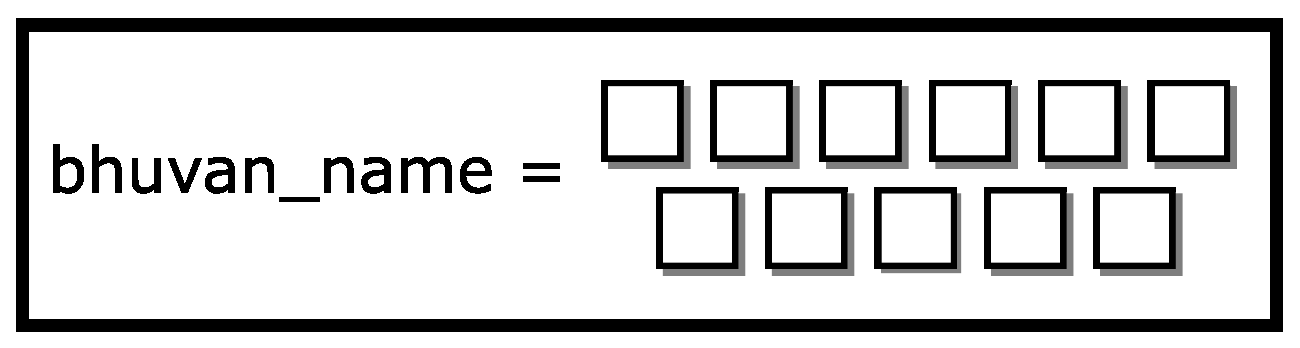
\includegraphics[width=.7\textwidth]{introc/drawings/memory_model_empty.eps}
\caption{Struct pointing to 11 empty boxes}
\end{figure}

So what happens when we assign length?
The first four boxes are filled with the value of the variable at length.
The rest of the space is left untouched.
We will assume that our machine is big endian.
This means that the least significant byte is last.

\begin{lstlisting}[language=C]
bhuvan_name->length = length;
\end{lstlisting}

\begin{figure}[H]
\centering
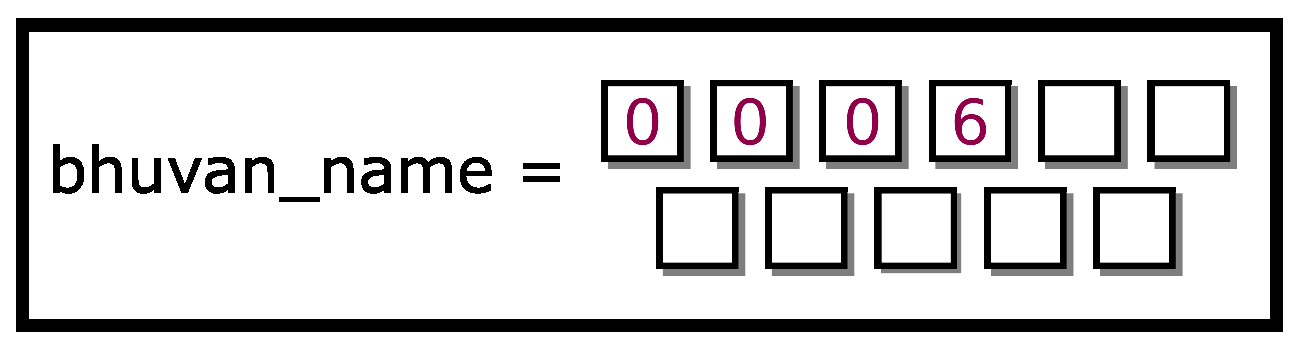
\includegraphics[width=.7\textwidth]{introc/drawings/memory_model_length.eps}
\caption{Struct pointing to 11 boxes, 4 filled with 0006, 7 junk}
\end{figure}

Now, we can write a string to the end of our struct with the following call.

\begin{minted}{C}
strcpy(bhuvan_name->c_str, to_convert);
\end{minted}

\begin{figure}[H]
\centering
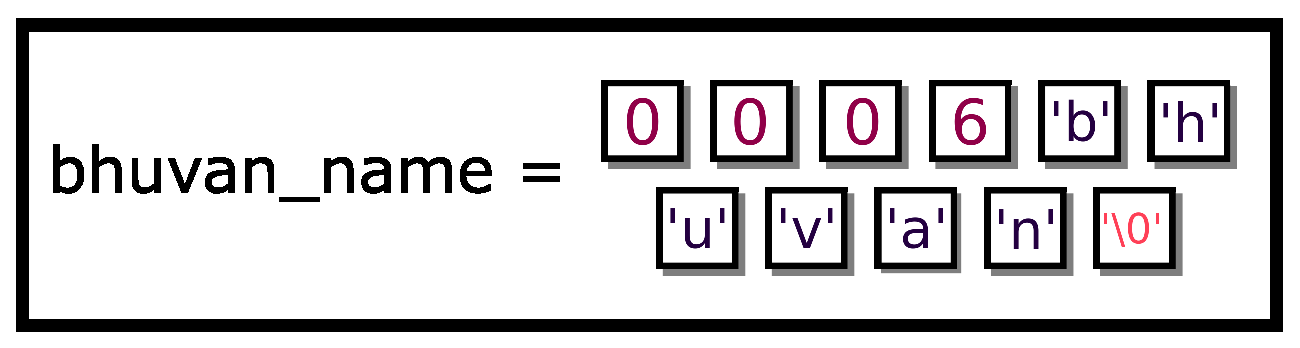
\includegraphics[width=.7\textwidth]{introc/drawings/memory_model_full.eps}
\caption{Struct pointing to 11 boxes, 4 filled with 0006, 7 the stirng ``bhuvan''}
\end{figure}

We can even do a sanity check to make sure that the strings are equal.

\begin{minted}{C}
strcmp(bhuvan_name->c_str, "bhuvan") == 0 //The strings are equal!
\end{minted}

What that zero length array does is point to the \textbf{end of the struct} this means that the compiler will leave room for all of the elements calculated with respect to their size on the operating system (ints, chars, etc).
The zero length array will take up no bytes of space.
Since structs are just continuous pieces of memory, we can allocate \textbf{more} space than required and use the extra space as a place to store extra bytes.
Although this seems like a parlor trick, it is an important optimization because to have a variable length string any other way, one would need to have two different memory allocation calls.
This is highly inefficient for doing something as common in programming as is string manipulation.

\subsubsection{Extra: Struct packing}

Structs may require something called \href{http://www.catb.org/esr/structure-packing/}{padding} (tutorial).
\textbf{We do not expect you to pack structs in this course, just know that it is there}.
This is because in the early days (and even now) loading an address in memory happens in 32-bit or 64-bit blocks.
This also meant requested addresses had to be multiples of block sizes.

\begin{lstlisting}[language=C]
struct picture{
  int height;
  pixel** data;
  int width;
  char* encoding;
}
\end{lstlisting}

You think the picture looks like this.
One box is four bytes.

\begin{figure}[H]
\centering
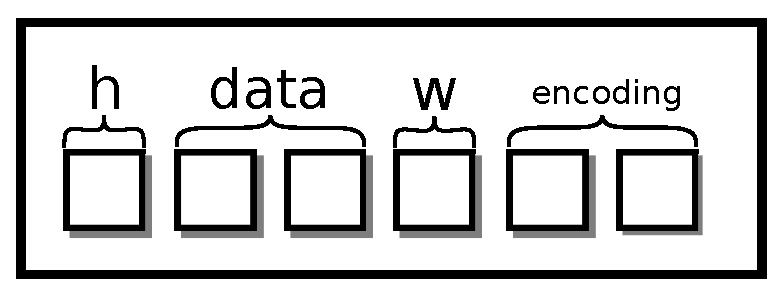
\includegraphics[width=.7\textwidth]{introc/drawings/struct_clean.eps}
\caption{Six box struct}
\label{fig:clean_struct}
\end{figure}

However, with struct packing, it would conceptually look like this:

\begin{lstlisting}[language=C]
struct picture{
  int height;
  char slop1[4];
  pixel** data;
  int width;
  char slop2[4];
  char* encoding;
}
\end{lstlisting}

Visually, we'd add two extra boxes to our diagram

\begin{figure}[H]
\centering
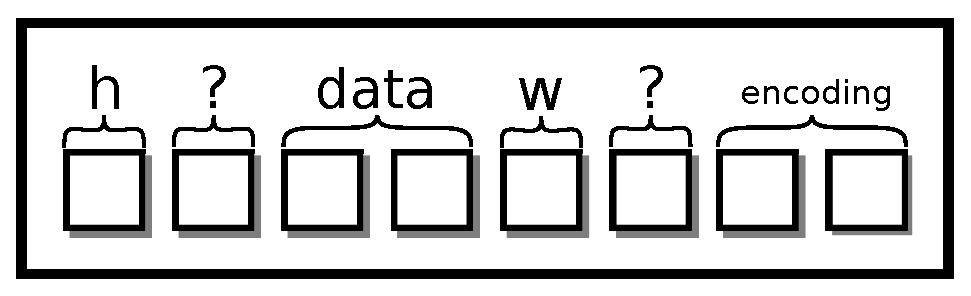
\includegraphics[width=.7\textwidth]{introc/drawings/struct_slop.eps}
\caption{Eight box struct, two boxes of slop}
\label{fig:sloppy_struct}
\end{figure}

This padding is common on a 64-bit system.
Other time, a processor supports unaligned access, leaving the compiler able to pack structs.
What does this mean?
We can have a variable start at a non-64-bit boundary.
The processor will figure out the rest.
To enable this, set an attribute.

\begin{lstlisting}[language=C]
struct __attribute__((packed, aligned(4))) picture{
  int height;
  pixel** data;
  int width;
  char* encoding;
}
\end{lstlisting}

Now our figure will look like the clean struct as in figure  \ref{fig:clean_struct}
But now, every time the processor needs to access \keyword{data} or \keyword{encoding},
two memory accesses are required.
A possible alternative is to reorder the struct.

\begin{lstlisting}[language=C]
struct picture{
  int height;
  int width;
  pixel** data;
  char* encoding;
}
\end{lstlisting}

\subsection{Strings in C}

In C, we have
\href{https://en.wikipedia.org/wiki/Null-terminated_string}{Null
	Terminated} strings rather than
\href{https://en.wikipedia.org/wiki/String_(computer_science)\#Length-prefixed}{Length
	Prefixed} for historical reasons.
For everyday programmers, remember to NUL terminate your string!
A string in C is defined as a bunch of bytes ended by `\0' or the NUL Byte.

\subsection{Places for strings}

Whenever you define a string literal - one in the form \keyword{char*\ str\ =\ "constant"} -- that string is stored in the \emph{data} section. Depending on your architecture, it is \textbf{read-only}, meaning that any attempt to modify the string will cause a SEGFAULT.
One can also declare strings to be either in the writable data segment or the stack. To do so, just specify a length for the string or put brackets instead of a pointer \keyword{char str[] = "mutable"} and put in the global scope or the function scope for the data segment or the stack respectively.
If one, however, \keyword{malloc}'s space, one can change that string to be whatever they want.
Forgetting to NUL terminate a string has a big effect on the strings! Bounds checking is important.
The heartbleed bug mentioned earlier in the book is partially because of this.

Strings in C are represented as characters in memory.
The end of the string includes a NUL (0) byte.
So "ABC" requires four(4) bytes.
The only way to find out the length of a C string is to keep reading memory until you find the NULL byte.
C characters are always exactly one byte each.

\subsubsection{String literals are constant}

A string literal is naturally constant.
Any write will cause the operating system to produce a SEGFAULT. 

\begin{lstlisting}[language=C]
char array[] = "Hi!"; // array contains a mutable copy
strcpy(array, "OK");

char *ptr = "Can't change me"; // ptr points to some immutable memory
strcpy(ptr, "Will not work");
\end{lstlisting}

String literals are character arrays stored in the code segment of the program, which is immutable.
Two string literals may share the same space in memory.
An example follows.

\begin{lstlisting}[language=C]
char *str1 = "Bhuvy likes books";
char *str2 = "Bhuvy likes books";
\end{lstlisting}

The strings pointed to by \keyword{str1} and \keyword{str2} may actually reside in the same location in memory.

Char arrays, however, contain the literal value which has been copied from the code segment into either the stack or static memory.
These following char arrays reside in different memory locations.

\begin{lstlisting}[language=C]
char arr1[] = "Bhuvy also likes to write";
char arr2[] = "Bhuvy also likes to write";
\end{lstlisting}

Here are some common ways to initialize a string include. Where do they reside in memory?

\begin{lstlisting}[language=C]
char *str = "ABC";
char str[] = "ABC";
char str[]={'A','B','C','\0'};
\end{lstlisting}

\begin{lstlisting}[language=C]
char ary[] = "Hello";
char *ptr = "Hello";
\end{lstlisting}

We can also print out the pointer and the contents of a C-string very easily. Here is some boilerplate code to illustrate this.

\begin{lstlisting}[language=C]
char ary[] = "Hello";
char *ptr = "Hello";
// Print out address and contents
printf("%p : %s\n", ary, ary);
printf("%p : %s\n", ptr, ptr);
\end{lstlisting}

As mentioned before, the char array is mutable, so we can change its contents.
Be careful to write within the bounds of the array.
C does \emph{not} do bounds checking at compile-time, but invalid reads/writes can get your program to crash.

\begin{lstlisting}[language=C]
strcpy(ary, "World"); // OK
strcpy(ptr, "World"); // NOT OK - Segmentation fault (crashes by default; unless SIGSEGV is blocked)
\end{lstlisting}

Unlike the array, however, we can change \keyword{ptr} to point to another piece of memory,

\begin{lstlisting}[language=C]
ptr = "World"; // OK!
ptr = ary; // OK!
ary = "World"; // NO won't compile
// ary is doomed to always refer to the original array.
printf("%p : %s\n", ptr, ptr);
strcpy(ptr, "World"); // OK because now ptr is pointing to mutable memory (the array)
\end{lstlisting}

Unlike pointers, that hold addresses to variables on the heap, or stack, char arrays (string literals) point to read-only memory located in the data section of the program. This means that pointers are more flexible than arrays, even though the name of an array is a pointer to its starting address.

In a more common case, pointers will point to heap memory in which case the memory referred to by the pointer \textbf{can} be modified.



\section{Pointers}

Pointers are variables that hold addresses.
These addresses have a numeric value, but usually, programmers are interested in the value of the contents at that memory address.
In this section, we will try to take you through a basic introduction to pointers.

\subsection{Pointer Basics}

\subsubsection{Declaring a Pointer}

A pointer refers to a memory address. The type of the pointer is useful -- it tells the compiler how many bytes need to be read/written and delineates the semantics for pointer arithmetic (addition and subtraction).

\begin{lstlisting}[language=C]
int *ptr1;
char *ptr2;
\end{lstlisting}

Due to C's syntax, an \keyword{int*} or any pointer is not actually its own type.
You have to precede each pointer variable with an asterisk.
As a common gotcha, the following

\begin{lstlisting}[language=C]
int* ptr3, ptr4;
\end{lstlisting}

Will only declare \keyword{*ptr3} as a pointer.
\keyword{ptr4} will actually be a regular int variable.
To fix this declaration, ensure the \keyword{*} precedes the pointer.

\begin{lstlisting}[language=C]
int *ptr3, *ptr4;
\end{lstlisting}

Keep this in mind for structs as well.
If one declares without a typedef, then the pointer goes after the type.

\begin{lstlisting}[language=C]
struct person *ptr3;
\end{lstlisting}

\subsubsection{Reading / Writing with pointers}

Let's say that \keyword{int\ *ptr} was declared.
For the sake of discussion, let us assume that \keyword{ptr} contains the memory address \keyword{0x1000}.
To write to the pointer, it must be dereferenced and assigned a value.

\begin{lstlisting}[language=C]
*ptr = 0; // Writes some memory.
\end{lstlisting}

What C does is take the type of the pointer which is an \keyword{int} and write \keyword{sizeof(int)} bytes from the start of the pointer, meaning that bytes \keyword{0x1000}, \keyword{0x1001}, \keyword{0x1002}, \keyword{0x1003} will all be zero.
The number of bytes written depends on the pointer type.
It is the same for all primitive types but structs are a little different.

Reading works roughly the same way, except you put the variable in the spot that it needs the value.

\begin{lstlisting}[language=C]
int double = *ptr * 2
\end{lstlisting}

Reading and writing to non-primitive types gets tricky.
The compilation unit - usually the file or a header - needs to have the size of the data structure readily available.
This means that opaque data structures can't be copied.
Here is an example of assigning a struct pointer:

\begin{lstlisting}[language=C]
#include <stdio.h>

typedef struct {
  int a1;
  int a2;
} pair;

int main() {
  pair obj;
  pair zeros;
  zeros.a1 = 0;
  zeros.a2 = 0;
  pair *ptr = &obj;
  obj.a1 = 1;
  obj.a2 = 2;
  *ptr = zeros;
  printf("a1: %d, a2: %d\n", ptr->a1, ptr->a2);
  return 0;
}
\end{lstlisting}

As for reading structure pointers, don't do it directly.
Instead, programmers create abstractions for creating, copying, and destroying structs.
If this sounds familiar, it is what C++ originally intended to do before the standards committee went off the deep end.

\subsection{Pointer Arithmetic}

In addition to adding to an integer, pointers can be added to.
However, the pointer type is used to determine how much to increment the pointer.
A pointer is moved over by the value added times the size of the underlying type.
For char pointers, this is trivial because characters are always one byte.

\begin{lstlisting}[language=C]
char *ptr = "Hello"; // ptr holds the memory location of 'H'
ptr += 2; // ptr now points to the first 'l''
\end{lstlisting}

If an int is 4 bytes then ptr+1 points to 4 bytes after whatever ptr is pointing at.

\begin{lstlisting}[language=C]
char *ptr = "ABCDEFGH";
int *bna = (int *) ptr;
bna +=1; // Would cause iterate by one integer space (i.e 4 bytes on some systems)
ptr = (char *) bna;
printf("%s", ptr);
\end{lstlisting}

Notice how only 'EFGH' is printed.
Why is that? Well as mentioned above, when performing 'bna+=1' we are increasing the **integer** pointer by 1, (translates to 4 bytes on most systems) which is equivalent to 4 characters (each character is only 1 byte)
Because pointer arithmetic in C is always automatically scaled by the size of the type that is pointed to, POSIX standards forbid arithmetic on void pointers.
Having said that, compilers will often treat the underlying type as \keyword{char}.
Here is a machine translation.
The following two pointer arithmetic operations are equal

\begin{lstlisting}[language=C]
int *ptr1 = ...;

// 1
int *offset = ptr1 + 4;

// 2
char *temp_ptr1 = (char*) ptr1;
int *offset = (int*)(temp_ptr1 + sizeof(int)*4);
\end{lstlisting}

\textbf{Every time you do pointer arithmetic, take a deep breath and make sure that you are shifting over the number of bytes you think you are shifting over.}

\subsection{So what is a void pointer?}

A void pointer is a pointer without a type.
Void pointers are used when either the datatype is unknown or when interfacing C code with other programming languages without APIs.
You can think of this as a raw pointer, or a memory address.
\keyword{malloc} by default returns a void pointer that can be safely promoted to any other type.

\begin{lstlisting}[language=C]
void *give_me_space = malloc(10);
char *string = give_me_space;
\end{lstlisting}

C automatically promotes \keyword{void*} to its appropriate type.
\keyword{gcc} and \keyword{clang} are not totally ISO C compliant, meaning that they will permit arithmetic on a void pointer.
They will treat it as a \keyword{char} pointer.
Do not do this because it is not portable - it is not guaranteed to work with all compilers!


\section{Common Bugs}

\subsection{Null Bytes}

What's wrong with this code?

\begin{lstlisting}[language=C]
void mystrcpy(char*dest, char* src) {
  // void means no return value
  while( *src ) { dest = src; src ++; dest++; }
}
\end{lstlisting}

In the above code it simply changes the dest pointer to point to source string.
Also the NUL bytes are not copied.
Here is a better version -

\begin{lstlisting}[language=C]
while( *src ) { *dest = *src; src ++; dest++; }
*dest = *src;
\end{lstlisting}

Note that it is also common to see the following kind of implementation, which does everything inside the expression test, including copying the NUL byte.
However, this is not good style, as a result of doing multiple operations in the same line.

\begin{lstlisting}[language=C]
while( (*dest++ = *src++ )) {};
\end{lstlisting}

\subsection{Double Frees}

A double free error is when a program accidentally attempt to free the same allocation twice.

\begin{lstlisting}[language=C]
int *p = malloc(sizeof(int));
free(p);

*p = 123; // Oops! - Dangling pointer! Writing to memory we don't own anymore

free(p); // Oops! - Double free!
\end{lstlisting}

The fix is first to write correct programs!
Secondly, it is a good habit to set pointers to NULL, once the memory has been freed.
This ensures that the pointer cannot be used incorrectly without the program crashing.

\begin{lstlisting}[language=C]
p = NULL; // No dangling pointers
\end{lstlisting}

\subsection{Returning pointers to automatic variables}

\begin{lstlisting}[language=C]
int *f() {
  int result = 42;
  static int imok;
  return &imok; // OK - static variables are not on the stack
  return &result; // Not OK
}
\end{lstlisting}

Automatic variables are bound to stack memory only for the lifetime of the function.
After the function returns, it is an error to continue to use the memory.

\subsection{Insufficient memory allocation}

\begin{lstlisting}[language=C]
struct User {
  char name[100];
};
typedef struct User user_t;

user_t *user = (user_t *) malloc(sizeof(user));
\end{lstlisting}

In the above example, we needed to allocate enough bytes for the struct.
Instead, we allocated enough bytes to hold a pointer.
Once we start using the user pointer we will corrupt memory.
The correct code is shown below.

\begin{lstlisting}[language=C]
struct User {
  char name[100];
};
typedef struct User user_t;

user_t * user = (user_t *) malloc(sizeof(user_t));
\end{lstlisting}

\subsection{Buffer overflow/ underflow}

A famous example: Heart Bleed performed a memcpy into a buffer that was of insufficient size.
A simple example: implement a strcpy and forget to add one to strlen, when determining the size of the memory required.

\begin{lstlisting}[language=C]
#define N (10)
int i = N, array[N];
for( ; i >= 0; i--) array[i] = i;
\end{lstlisting}

C does not check if pointers are valid.
The above example writes into \keyword{array[10]} which is outside the array bounds.
This can cause memory corruption because that memory location is probably being used for something else.
In practice, this can be harder to spot because the overflow/underflow may occur in a library call.
Here is our old friend gets.

\begin{lstlisting}[language=C]
gets(array); // Let's hope the input is shorter than my array!
\end{lstlisting}


\subsection{Strings require strlen(s)+1 bytes}

Every string must have a null byte after the last characters.
To store the string ``Hi'' it takes 3 bytes: [H] [i] [\backslash 0].

\begin{lstlisting}[language=C]
char *strdup(const char *input) {  /* return a copy of 'input' */
  char *copy;
  copy = malloc(sizeof(char*));     /* nope! this allocates space for a pointer, not a string */
  copy = malloc(strlen(input));     /* Almost...but what about the null terminator? */
  copy = malloc(strlen(input) + 1); /* That's right. */
  strcpy(copy, input);   /* strcpy will provide the null terminator */
  return copy;
}
\end{lstlisting}

\subsection{Using uninitialized variables}

\begin{lstlisting}[language=C]
int myfunction() {
  int x;
  int y = x + 2;
  ...
\end{lstlisting}

Automatic variables hold garbage or bit pattern that happened to be in memory or register.
It is an error to assume that it will always be initialized to zero.

\subsection{Assuming Uninitialized memory will be zeroed}

\begin{lstlisting}[language=C]
void myfunct() {
  char array[10];
  char *p = malloc(10);
\end{lstlisting}

Automatic (temporary variables) are not automatically initialized to zero.
Heap allocations using malloc are not automatically initialized to zero.

\section{Logic and Program flow mistakes}

These are a set of mistakes that may or may not make sense within the context of the program.

\subsection{Equal vs. Equality}

Confusingly in C, the assignment operator also returns the assigned value.
Most of the time it is ignored.
We can use it to initialize multiple things on the same line.

\begin{lstlisting}[language=C]
  int p1, p2;
  p1 = p2 = 0;
\end{lstlisting}

More confusingly, if we forget an equals sign in the equality operator we will end up assigning that variable.
Most of the time this isn't what we want to do.

\begin{lstlisting}[language=C]
int answer = 3; // Will print out the answer.
if (answer = 42) { printf("I've solved the answer! It's %d", answer);}
\end{lstlisting}

The quick way to fix that is to get in the habit of putting constants first.
This mistake is common enough in while loop conditions, that most modern programming languages do not let you assign in a while loop without some kind of warning, and some do not allow it at all.

\begin{lstlisting}[language=C]
if (42 = answer) { printf("I've solved the answer! It's %d", answer);}
\end{lstlisting}

There are cases where we want to do it.
A common example is getline.

\begin{lstlisting}[language=C]
while ((nread = getline(&line, &len, stream)) != -1)
\end{lstlisting}

This piece of code calls getline, and assigns the return value or the number of bytes read to nread.
It also in the same line checks if that value is -1 and if so terminates the loop.
It is always good practice to put parenthesis around any assignment condition.

\subsection{Undeclared or incorrectly prototyped functions}

You may see code do something like this.

\begin{lstlisting}[language=C]
time_t start = time();
\end{lstlisting}

The system function `time' actually takes a parameter a pointer to some memory that can receive the time\_t structure or NULL.
The compiler did not catch this error because the programmer did not provide a valid function prototype by including \keyword{time.h}.

More confusingly this could compile, work for decades and then crash.
The reason for that is that time would be found at link time, not compile time in the C standard library which almost surely is already in memory.
Since a parameter isn't being passed, we are hoping the arguments on the stack (any garbage) is zeroed out because if it isn't, time will try to write the result of the function to that garbage which will cause the program to SEGFAULT.

\subsection{Extra Semicolons}

This is a pretty simple one, don't put semicolons when not needed.

\begin{lstlisting}[language=C]
for(int i = 0; i < 5; i++) ; printf("I'm printed once");
while(x < 10); x++ ; // X is never incremented
\end{lstlisting}

However, the following code is perfectly OK.

\begin{lstlisting}[language=C]
for(int i = 0; i < 5; i++){
    printf("%d\n", i);;;;;;;;;;;;;
}
\end{lstlisting}

It is OK to have this kind of code, because the C language uses semicolons (;) to separate statements.
If there is no statement in between semicolons, then there is nothing to do and the compiler moves on to the next statement
To save a lot of confusion, \textbf{always using braces.}
It increases the number of lines of code, which is a great productivity metric.




\section{Topics}

\begin{itemize}
	\tightlist
	\item
	      C-strings representation
	\item
	      C-strings as pointers
	\item
	      char p{[}{]}vs char* p
	\item
	      Simple C string functions (strcmp, strcat, strcpy)
	\item
	      sizeof char
	\item
	      sizeof x vs x*
	\item
	      Heap memory lifetime
	\item
	      Calls to heap allocation
	\item
	      Dereferencing pointers
	\item
	      Address-of operator
	\item
	      Pointer arithmetic
	\item
	      String duplication
	\item
	      String truncation
	\item
	      double-free error
	\item
	      String literals
	\item
	      Print formatting.
	\item
	      memory out of bounds errors
	\item
	      static memory
	\item
	      file input / output. POSIX vs. C library
	\item
	      C input output: fprintf and printf
	\item
	      POSIX file IO (read, write, open)
	\item
	      Buffering of stdout
\end{itemize}

\section{Questions/Exercises}

\begin{itemize}
	\item
	      What does the following print out?

	      \begin{lstlisting}[language=C]
int main(){
fprintf(stderr, "Hello ");
fprintf(stdout, "It's a small ");
fprintf(stderr, "World\n");
fprintf(stdout, "place\n");
return 0;
}
\end{lstlisting}
	\item
	      What are the differences between the following two declarations? What
	      does \keyword{sizeof} return for one of them?

	      \begin{lstlisting}[language=C]
char str1[] = "first one";
char *str2 = "another one";
\end{lstlisting}
	\item
	      What is a string in C?
	\item
	      Code up a simple \keyword{my\_strcmp}. How about \keyword{my\_strcat}, \keyword{my\_strcpy}, or \keyword{my\_strdup}? Bonus: Code the functions while only going through the strings \emph{once}.
	\item
	      What should each of the following lines usually return?

	      \begin{lstlisting}[language=C]
int *ptr;
sizeof(ptr);
sizeof(*ptr);
\end{lstlisting}
	\item
	      What is \keyword{malloc}? How is it different from \keyword{calloc}. Once memory is allocated how can we use \keyword{realloc}?
	\item
	      What is the \keyword{\&} operator? How about \keyword{*}?
	\item
	      Pointer Arithmetic. Assume the following addresses. What are the following shifts?

	      \begin{lstlisting}[language=C]
char** ptr = malloc(10); //0x100
ptr[0] = malloc(20); //0x200
ptr[1] = malloc(20); //0x300
\end{lstlisting}

	      \begin{itemize}
		      \tightlist
		      \item
		            \keyword{ptr\ +\ 2}
		      \item
		            \keyword{ptr\ +\ 4}
		      \item
		            \keyword{ptr{[}0{]}\ +\ 4}
		      \item
		            \keyword{ptr{[}1{]}\ +\ 2000}
		      \item
		            \keyword{*((int)(ptr\ +\ 1))\ +\ 3}
	      \end{itemize}
	\item
	      How do we prevent double free errors?
	\item
	      What is the printf specifier to print a string, \keyword{int}, or
	      \keyword{char}?
	\item
	      Is the following code valid? Why? Where is \keyword{output}
	      located?

	      \begin{lstlisting}[language=C]
char *foo(int var){
static char output[20];
snprintf(output, 20, "%d", var);
return output;
}
\end{lstlisting}
	\item
	      Write a function that accepts a path as a string, and opens that file, prints the file contents 40 bytes at a time but, every other print reverses the string (try using the POSIX API for this).
	\item
	      What are some differences between the POSIX file descriptor model and C's \keyword{FILE*} (i.e. what function calls are used and which is buffered)? Does POSIX use C's \keyword{FILE*} internally or vice versa?
\end{itemize}

\section{Rapid Fire: Pointer Arithmetic}

Pointer arithmetic is important!
Take a deep breath and figure out how many bytes each operation moves a pointer.
The following is a rapid fire section.
We'll use the following definitions:

\begin{lstlisting}[language=C]
int *int_; // sizeof(int) == 4;
long *long_; // sizeof(long) == 8;
char *char_;
int *short_; //sizeof(short) == 2;
int **int_ptr; // sizeof(int*) == 8;
\end{lstlisting}

How many bytes are moved over from the following additions?

\begin{enumerate}
\item \keyword{int\_ + 1}
\item \keyword{long\_ + 7}
\item \keyword{short\_ - 6}
\item \keyword{short\_ - sizeof(long)}
\item \keyword{long\_ - sizeof(long) + sizeof(int\_)}
\item \keyword{long\_ - sizeof(long) / sizeof(int)}
\item \keyword{(char*)(int\_ptr + sizeof(long)) + sizeof(int\_)}
\end{enumerate}

\subsection{Rapid Fire Solutions}

\begin{enumerate}
\item 4
\item 56
\item -12
\item -16
\item 0
\item -16
\item 72
\end{enumerate}

\bibliographystyle{plainnat}
\bibliography{introc/introc}
